% Title: glps_renderer figure
% Creator: GL2PS 1.3.8, (C) 1999-2012 C. Geuzaine
% For: Octave
% CreationDate: Wed Nov 19 17:21:25 2014
\setlength{\unitlength}{1pt}
\begin{picture}(0,0)
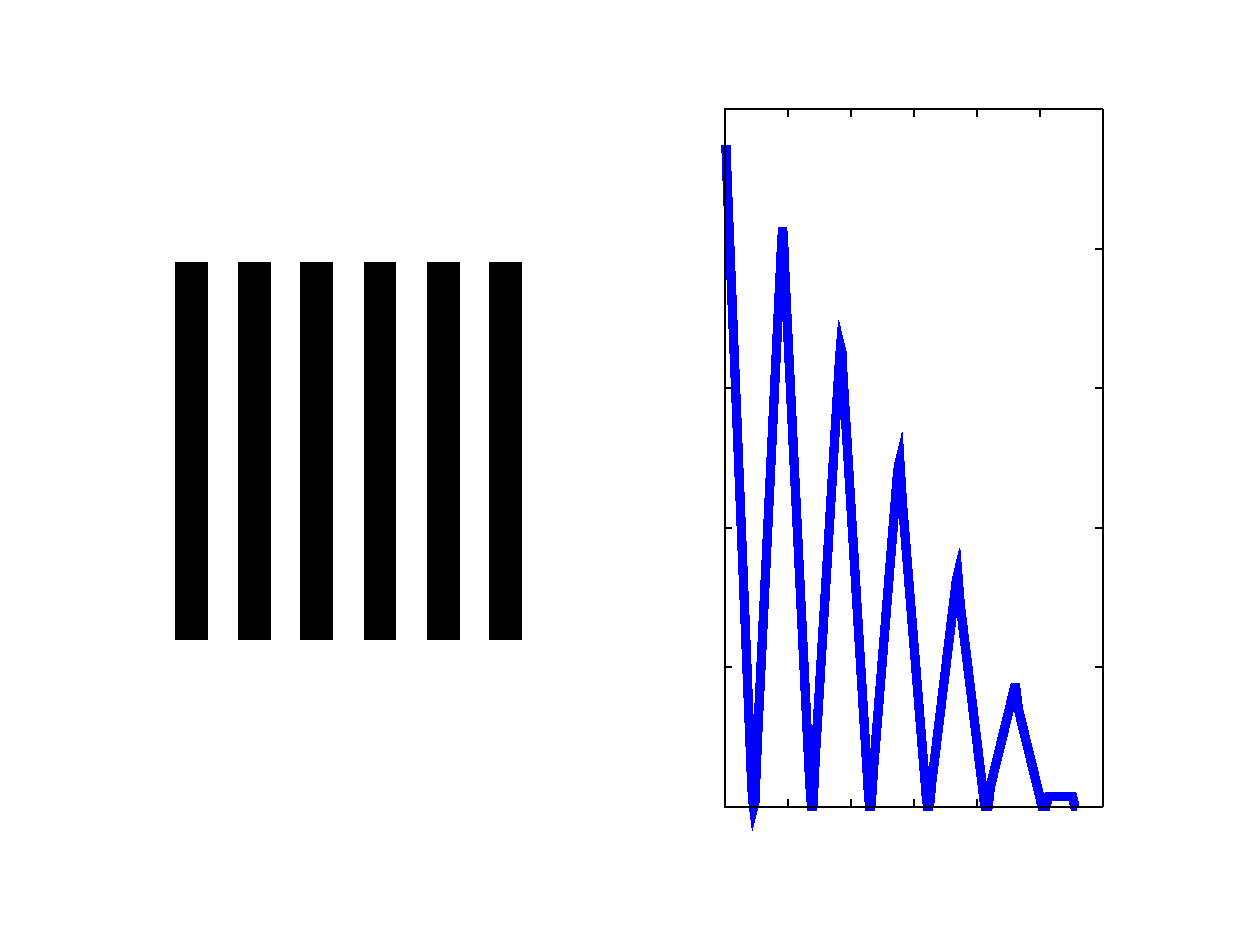
\includegraphics{data/tex/periode-inc}
\end{picture}%
\begin{picture}(450,432)(0,0)
\fontsize{10}{0}
\selectfont\put(165.6,324.28){\makebox(0,0)[b]{\textcolor[rgb]{0,0,0}{{Motif original}}}}
\fontsize{10}{0}
\selectfont\put(339.84,47.6068){\makebox(0,0)[t]{\textcolor[rgb]{0,0,0}{{0}}}}
\fontsize{10}{0}
\selectfont\put(370.08,47.6068){\makebox(0,0)[t]{\textcolor[rgb]{0,0,0}{{50}}}}
\fontsize{10}{0}
\selectfont\put(400.32,47.6068){\makebox(0,0)[t]{\textcolor[rgb]{0,0,0}{{100}}}}
\fontsize{10}{0}
\selectfont\put(430.56,47.6068){\makebox(0,0)[t]{\textcolor[rgb]{0,0,0}{{150}}}}
\fontsize{10}{0}
\selectfont\put(460.8,47.6068){\makebox(0,0)[t]{\textcolor[rgb]{0,0,0}{{200}}}}
\fontsize{10}{0}
\selectfont\put(491.04,47.6068){\makebox(0,0)[t]{\textcolor[rgb]{0,0,0}{{250}}}}
\fontsize{10}{0}
\selectfont\put(521.28,47.6068){\makebox(0,0)[t]{\textcolor[rgb]{0,0,0}{{300}}}}
\fontsize{10}{0}
\selectfont\put(334.828,52.6037){\makebox(0,0)[r]{\textcolor[rgb]{0,0,0}{{0}}}}
\fontsize{10}{0}
\selectfont\put(334.828,119.563){\makebox(0,0)[r]{\textcolor[rgb]{0,0,0}{{0.2}}}}
\fontsize{10}{0}
\selectfont\put(334.828,186.522){\makebox(0,0)[r]{\textcolor[rgb]{0,0,0}{{0.4}}}}
\fontsize{10}{0}
\selectfont\put(334.828,253.482){\makebox(0,0)[r]{\textcolor[rgb]{0,0,0}{{0.6}}}}
\fontsize{10}{0}
\selectfont\put(334.828,320.441){\makebox(0,0)[r]{\textcolor[rgb]{0,0,0}{{0.8}}}}
\fontsize{10}{0}
\selectfont\put(334.828,387.4){\makebox(0,0)[r]{\textcolor[rgb]{0,0,0}{{1}}}}
\fontsize{10}{0}
\selectfont\put(430.56,34.6068){\makebox(0,0)[t]{\textcolor[rgb]{0,0,0}{{n : distance les deux points}}}}
\fontsize{10}{0}
\selectfont\put(430.56,397.4){\makebox(0,0)[b]{\textcolor[rgb]{0,0,0}{{fonction de correlation}}}}
\end{picture}
